\chapter{Приложение}
\label{ch:appendix}

\section{Приложение А. Схема установки}

    Схема установки, используемой в работе, приведена на рис. 1. На оси полой цилиндрической трубки с внутренним диаметром $2r_0 \sim 1$ см размещена металлическая нить диаметром $2r_1 \sim 0,05$ мм и длиной $L \sim 40$ см. Полость трубки заполнена воздухом (полость через небольшое отверстие сообщается с атмосферой). Стенки трубки помещены в кожух, через который пропускается вода из термостата, так что их температура $t_0$ поддерживается постоянной. Для предотвращения конвекции трубка расположена вертикально.

    Металлическая нить служит как источником тепла, так и датчиком температуры (термометром сопротивления). По пропускаемому через нить постоянному току $I$ и напряжению $U$ на ней вычисляется мощность нагрева по закону Джоуля–Ленца: $Q = UI$, и сопротивление нити по закону Ома: $R = \dfrac{U}{I}$.

    Сопротивление нити является однозначной функцией её температуры $R (t)$.
    Эта зависимость может быть измерена с помощью термостата по экстраполяции мощности нагрева к нулю $Q \rightarrow 0$, когда температура нити и стенок совпадают $t_1 \approx t_0$. Альтернативно, если материал нити известен, зависимость его удельного сопротивления от температуры может быть найдена по справочным данным.

    Параметры установки $ ln \frac{r_0}{r_1} = 5$,  $L = (400 \pm 2)~\text{мм}$,  $R_\text{н} \sim 20~\text{Ом}$,  $k_\text{в} \sim 25 * 10^{-3}~\frac{\text{Вт}}{\text{м}*\text{с}} $.

\section{Приложение Б. Вывод расчётной формулы k для используемой установки}

    Рассмотрим стационарную теплопроводность в цилиндрической геометрии (см. рис. 1). Пусть тонкая нить радиусом $r_1$ и длиной $L$ помещена на оси цилиндра радиусом $r_0$. Температура стенок цилиндра $T_0$ поддерживается постоянной. Пусть в нити выделяется некоторая тепловая мощность $Q$ [Вт]. Если цилиндр длинный ($L$ >> $r_0$), можно пренебречь теплоотводом через его торцы. Тогда все параметры газа можно считать зависящими только от расстояния до оси системы $r$, а поток тепла $\overline{q}$ направленным строго радиально. Вместо (1) имеем скалярное уравнение

    \[q = - k \frac{dT}{dr}\].

    В стационарном состоянии полный поток тепла через любую цилиндрическую поверхность радиуса $r$ площадью $S = 2\uppi rL$ должен быть одинаков и равен $Q = qS$:

    \[Q = - 2\uppi rL \cdot k \frac{dT}{dr} = const\].

    Если перепад температуры $\Delta T = T_1 - T_0$ между нитью и стенками цилиндра мал ($\Delta T << T_0$), то можно пренебречь изменением теплопроводности от температуры в пределах системы, положив $k \approx k(T_0)$. Тогда разделяя переменные и интегрируя от радиуса нити до радиуса колбы, получим

    \[Q = \frac{2 \uppi L}{\ln{r_0/r_1}} k \Delta T\]. 

\section{Приложение В. Методика измерения температуры}

    Принципиально неустранимая систематическая ошибка измерения температуры с помощью термометра сопротивления возникает из-за необходимости пропускать через резистор (нить) измерительный ток. Чем этот ток выше, тем с большей точностью будет измерен как он сам, так и напряжение. Однако при этом квадратично возрастает выделяющаяся на  резисторе мощность $Q = UI = I^2R$. Следовательно, температура резистора становится выше, чем у объекта, температуру которого надо измерить. Измерения же при малых токах не дают достаточной точности (в частности, из-за существенного вклада термоэлектрических явлений в проводниках и контактах). Эта проблема решается построением нагрузочной кривой - зависимости измеряемого сопротивления $R$ от выделяющейся в нём мощности $R(Q)$, с последующей экстраполяцией к нулевой мощности $Q \to 0$ для определения сопротивления $R_0 = R(0)$, при котором его температура равна температуре измеряемого объекта. Кроме того, в данной работе измерение нагрузочных кривых позволяет в ходе эксперимента получить температурную зависимость сопротивления нити, так как при $Q \to 0$ температура нити равна температуре термостата ($T \approx T_0$). В исследуемом интервале температур ($20-80 \celsius$) зависимость сопротивления от температуры можно с хорошей точностью аппроксимировать линейной функцией:

    \begin{align}
        R(T) = R_{273} \cdot (1 + \alpha T) \label{RT}
    \end{align}

    где $\alpha = \dfrac{1}{R_{273}} \dfrac{dR}{dT}$ - температурный коэффициент сопротивления материала.

    Приняли максимально допустимый перегрев нити относительно термостата равным $\Delta t_{max} = 30 \celsius$. По формуле (\ref{Q}) оценили максимальную мощность нагрева $Q_{max} \approx 370~\text{мВт}$. Также оценили максимальные ток и напряжение $I_{max} \approx 2.91~\text{В}$; $U_{max} \approx 128~\text{мА}$. В ходе работы они не превышались.

    В процессе измерения контролировали постоянство температуры термостата. Его показания оставались стабильными. Провели измерения ещё для 5 температур до $80~^oC$.

    %Второстепенное в приложение. Важна именно зависимость температуры.

\section{Приложение Г. Измерение зависимости сопротивления нити от подаваемой на неё мощности}

    Измерения провели для 10 значений тока через нить. Подобрали значения тока так, чтобы мощность возрастала равномерно. В соответствии с формулой $Q = \frac{I^2}{R_\text{н}}$ мощность пропорциональна квадрату напряжения (изменением сопротивления для данной оценки пренебрежём).

    Напряжение наращивали постепенно, уменьшая сопротивление моста. Перед каждой фиксацией показаний ожидали установления теплового равновесия ($\sim 30~\text{с}$). При измерениях сразу вычисляем $R_\text{н}$ и $Q$.

    Результаты измерений см. в Приложении Е.

    Нашли ток в цепи по формуле: $I = \frac{U}{R}$, где $R$ -  сопротивление моста, $I$ - ток через систему, $U_e$ - напряжение в цепи. Мощность нагрева вычисляется по закону Джоуля-Ленца: $Q = U * I$.

    \begin{figure}[ht]
        \center{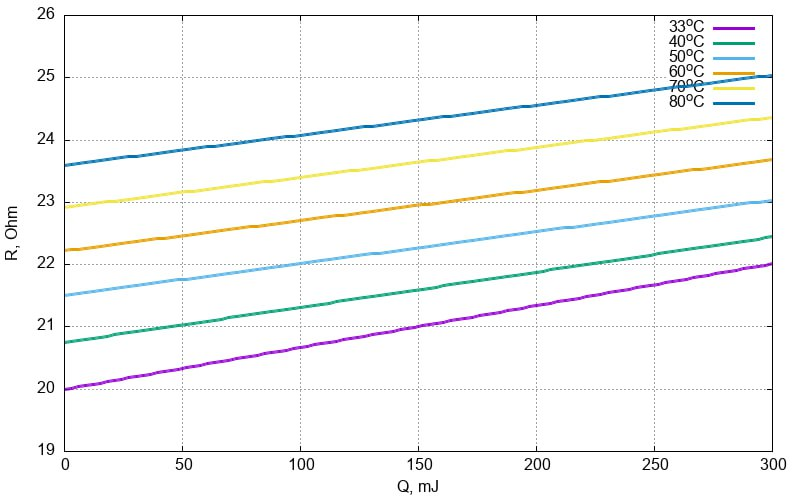
\includegraphics[scale=0.5]{img/raw.png}}
        \begin{center}       
        Рис. 5. График зависимости $R_\text{н}(Q)$ для разных температур термостата (от $33$ до $80 \celsius$) 
        \end{center}
        \label{RQ_graph}
    \end{figure}

    Нашли коэффициенты наклона и точки пересечения графиков зависимости $R_\text{н}(Q)$ с осью $R$, результаты в таблице:

    \begin{table}[!ht]
        \begin{minipage}{\linewidth}
            \centering
            \begin{tabular}{|c|c|c|}
            \hline

            № & $\frac{dR}{dQ}$, $\frac{\text{Вт}}{\text{Ом}} \cdot 10^{-6}$ & $R_0, \text{Ом}$ \\ \hline
                1	& $6.72  \pm 0.26$	& 19.998 \\ \hline
                2	& $5.65  \pm 0.26$	& 20.751 \\ \hline
                3	& $5.10  \pm 0.11$	& 21.507 \\ \hline
                4	& $4.87  \pm 0.06$	& 22.221 \\ \hline
                5	& $4.820 \pm 0.012$	& 22.92  \\ \hline
                6	& $4.817 \pm 0.012$ & 23.60  \\ \hline

            \end{tabular}
                \caption{Коэффициенты наклона и точки пересечения графиков с осью}
            \label{table_dR/dQ}
        \end{minipage}
    \end{table}

    Коэффициенты наклона уменьшаются с ростом температуры. Это можно объяснить конвекцией воздуха внутри трубы. С ростом температуры влияние этого явления увеличивается.

\section{Приложение Д. Зависимость сопротивления нити от температуры}

    Построили график $R_0(T)$. Методика измерения температуры приведена в Приложении В.

    \begin{figure}[ht]
        \center{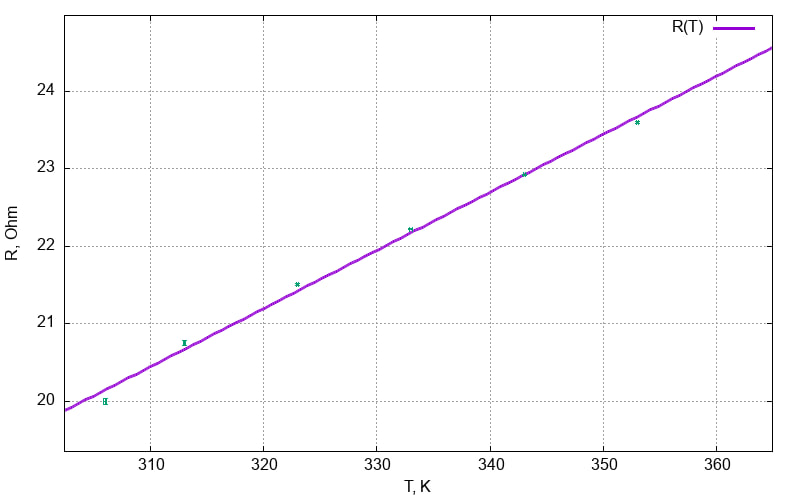
\includegraphics[scale=0.5]{img/ROT.png}}
        \begin{center}       
        Рис. 6. График зависимости $R_0(T)$
        \end{center}
        \label{RT_graph}
    \end{figure}

    Получили коэффициент наклона линейной зависимости: $\frac{dR}{dT} = (4.27 \pm 0.031) \cdot 10^{-2} \frac{\text{Ом}}{\text{К}}$

\section{Приложение Е. Результаты измерений}

    \begin{table}[!ht]
        \begin{minipage}{.42\linewidth}
            \centering
            \begin{tabular}{|c|c|c|c|}
                \hline

                $I, \text{мА}$ & $U, \text{мВ}$ &  $R_\text{н}, \text{Ом}$ & $Q, \text{Вт}$\\ \hline
                13,10	& 255	& 19,4656	& 3,3405 \\ \hline
                38,89	& 769	& 19,7737	& 29,90641 \\ \hline
                52,86	& 1090	& 20,6205	& 57,6174 \\ \hline
                62,78	& 1300	& 20,7072	& 81,614 \\ \hline
                70,62	& 1470	& 20,8156	& 103,8114 \\ \hline
                77,07	& 1620	& 21,0199	& 124,8534 \\ \hline
                82,68	& 1740	& 21,0450	& 143,8632 \\ \hline
                87,57	& 1850	& 21,1260	& 162,0045 \\ \hline
                91,73	& 1950	& 21,2580	& 178,8735 \\ \hline
                95,70	& 2040	& 21,3166	& 195,228 \\ \hline
                99,21	& 2130	& 21,4696	& 211,3173 \\ \hline

            \end{tabular}
            \caption{   Измерения при температуре термостата $33^oC$}
            \label{table_61}
        \end{minipage}
    \end{table}
    \begin{table}[!ht]
        \begin{minipage}{.42\linewidth}
            \centering
            \begin{tabular}{|c|c|c|c|}
                \hline

                $I, \text{мА}$ & $U, \text{мВ}$ &  $R_\text{н}, \text{Ом}$ & $Q, \text{Вт}$\\ \hline
                13,07	& 270	& 20,6580	& 3,5289 \\ \hline
                38,61	& 810	& 20,9790	& 31,2741 \\ \hline
                52,36	& 1105	& 21,1039	& 57,8578 \\ \hline
                62,07	& 1320	& 21,2663	& 81,9324 \\ \hline
                69,75	& 1490	& 21,3620	& 103,9275 \\ \hline
                76,00   & 1630	& 21,4474	& 123,88 \\ \hline
                81,52	& 1760	& 21,5898	& 143,4752 \\ \hline
                86,23	& 1870	& 21,6862	& 161,2501 \\ \hline
                90,27	& 1960	& 21,7126	& 176,9292 \\ \hline
                94,13	& 2050	& 21,7784	& 192,9665 \\ \hline
                97,56	& 2140	& 21,9352	& 208,7784 \\ \hline

            \end{tabular}
                \caption{Измерения при температуре термостата $40^oC$}
            \label{table_80}
        \end{minipage}
    \end{table}

    \begin{table}[!ht]
        \begin{minipage}{.42\linewidth}
            \centering
            \begin{tabular}{|c|c|c|c|}
                \hline

                $I, \text{мА}$ & $U, \text{мВ}$ &  $R_\text{н}, \text{Ом}$ & $Q, \text{Вт}$\\ \hline
                13,03	& 280	& 21,4889	& 3,6484 \\ \hline
                32,23	& 828	& 21,6904	& 26,68644 \\ \hline
                51,66	& 1126	& 21,7964	& 58,16916 \\ \hline
                61,09	& 1339	& 21,9185	& 81,79951 \\ \hline
                68,53	& 1510	& 22,0341	& 103,4803 \\ \hline
                74,58	& 1651	& 22,1373	& 123,13158 \\ \hline
                79,88	& 1776	& 22,2334	& 141,86688 \\ \hline
                84,43	& 1884	& 22,3143	& 159,06612 \\ \hline
                88,32	& 1978	& 22,3958	& 174,69696 \\ \hline
                92,01	& 2068	& 22,4758	& 190,27668 \\ \hline
                95,34	& 2150	& 22,5509	& 204,981 \\ \hline

            \end{tabular}
            \caption{Измерения при температуре термостата $50^oC$}
            \label{table_61}
        \end{minipage}
    \end{table}
    \begin{table}[!ht]
        \begin{minipage}{.42\linewidth}
            \centering
            \begin{tabular}{|c|c|c|c|}
                \hline

                $I, \text{мА}$ & $U, \text{мВ}$ &  $R_\text{н}, \text{Ом}$ & $Q, \text{Вт}$\\ \hline
                12,98	& 289	& 22,2650	& 3,75122 \\ \hline
                37,96	& 849	& 22,3656	& 32,22804 \\ \hline
                50,98	& 1147	& 22,4990	& 58,47406 \\ \hline
                60,15	& 1360	& 22,6101	& 81,804 \\ \hline
                67,36	& 1530	& 22,7138	& 103,0608 \\ \hline
                73,20	& 1670	& 22,8142	& 122,244 \\ \hline
                78,33	& 1794	& 22,9031	& 140,52402 \\ \hline
                82,67	& 1900	& 22,9829	& 157,073 \\ \hline
                86,44	& 1994	& 23,0680	& 172,36136 \\ \hline
                89,99	& 2082	& 23,1359	& 187,35918 \\ \hline
                93,19	& 2163	& 23,2106	& 201,56997 \\ \hline

            \end{tabular}
            \caption{Измерения при температуре термостата $60^oC$}
            \label{table_80}
        \end{minipage}
    \end{table}

    \begin{table}[!ht]
        \begin{minipage}{.42\linewidth}
            \centering
            \begin{tabular}{|c|c|c|c|}
                \hline

                $I, \text{мА}$ & $U, \text{мВ}$ &  $R_\text{н}, \text{Ом}$ & $Q, \text{Вт}$\\ \hline
                12,94	& 297	& 22,952	& 3,84318 \\ \hline
                37,44	& 864	& 23,076	& 32,34816 \\ \hline
                50,32	& 1167	& 23,191	& 58,72344 \\ \hline
                59,25	& 1381	& 23,308	& 81,82425 \\ \hline
                66,22	& 1550	& 23,406	& 102,641 \\ \hline
                71,87	& 1689	& 23,500	& 121,38843 \\ \hline
                76,80	& 1812	& 23,593	& 139,1616 \\ \hline
                81,02	& 1917	& 23,660	& 155,31534 \\ \hline
                84,62	& 2008	& 23,729	& 169,91696 \\ \hline
                88,03	& 2095	& 23,798    & 184,42285 \\ \hline
                91,11	& 2074	& 23,863	& 188,96214 \\ \hline

            \end{tabular}
            \caption{Измерения при температуре термостата $70^oC$}
            \label{table_61}
        \end{minipage}
    \end{table}
    \begin{table}[!ht]
        \begin{minipage}{.42\linewidth}
            \centering
            \begin{tabular}{|c|c|c|c|}
                \hline

                $I, \text{мА}$ & $U, \text{мВ}$ &  $R_\text{н}, \text{Ом}$ & $Q, \text{Вт}$\\ \hline
                12,89	& 305	& 23,652	& 3,932975 \\ \hline
                37,13	& 880	& 23,700	& 32,6744 \\ \hline
                49,67	& 1187	& 23,897    & 58,95829 \\ \hline
                59,62	& 1430	& 23,985	& 85,2566 \\ \hline
                65,12	& 1569	& 24,094	& 102,17328 \\ \hline
                70,58	& 1707	& 24,185	& 120,48006 \\ \hline
                75,36	& 1829	& 24,270	& 137,83344 \\ \hline
                79,41	& 1933	& 24,342	& 153,49953 \\ \hline
                82,88	& 2023	& 24,408	& 167,66624 \\ \hline
                86,16	& 2108	& 24,466	& 181,62528 \\ \hline
                89,11	& 2186	& 24,531	& 194,79446 \\ \hline

            \end{tabular}
            \caption{Измерения при температуре термостата $80^oC$}
            \label{table_80}
        \end{minipage}
    \end{table}